\documentclass[fleqn,a4paper,12pt]{article}
\usepackage[top=1in, bottom=1in, left=1in, right=1in]{geometry}



\title{Machine Learning Homework 3}
\date{}

\setcounter{section}{2}

\usepackage{listings}

\usepackage{amsmath}
\usepackage{amssymb}


\usepackage{mathspec}
\setmainfont{Noto Serif CJK TC}
% \setmathsfont(Digits,Latin,Greek)[Numbers={Lining,Proportional}]{DejaVu Math TeX Gyre}
\newfontfamily\ZhFont{Noto Serif CJK TC}
\newfontfamily\SmallFont[Scale=0.8]{Droid Sans}
% \newfontfamily\SmallSmallFont[Scale=0.7]{Noto Serif CJK}
\usepackage{fancyhdr}
\usepackage{lastpage}
\pagestyle{fancy}
\fancyhf{}
\rhead{B03902072\ZhFont{江廷睿}}
\lhead{Machine Learning Homework 3}
\rfoot{\thepage / \pageref{LastPage}}


\usepackage{graphicx}
\usepackage{caption}
\usepackage{subcaption}
\usepackage{float}

\begin{document}
\maketitle
\thispagestyle{fancy}

\subsection*{P1: Build Convolution Neural Network}

\subsubsection*{Image Preprocess}

First center the image pixelwise so each pixel has zero mean. Then divide each pixel with maximum absolute value among all pixels, so all value of all the pixels are within [-1, 1] \cite{cs221_project}.

\subsubsection*{CNN Structure}

The final structure of my CNN is

\begin{itemize}
\item
  Input (48, 48, 1)
\item
  Image Augmentation (48, 48, 1): Augmentate images in batch by randomly
  \begin{itemize}
  \item rotating in (-30, 30) degrees.
  \item flipping horizontally.
  \item shifting horizontally and vertically in (-4.8, 4.8) pixels.
  \item zooming by (0.8, 1.2)
  \end{itemize}
\item
  Conv2d (24, 24, 32): Conv2d with kernel size (3, 3), stride 1, same padding, followed by batch normalization, leaky ReLU, max pooling with kernel size (2, 2), stride 1.
\item
  Conv2d (12, 12, 64): Conv2d with kernel size (3, 3), stride 1, same padding, followed by batch normalization, leaky ReLU, max pooling with kernel size (2, 2), stride 1.
\item
  Dropout with rate 0.1
\item
  Conv2d (6, 6, 128): Conv2d with kernel size (3, 3), stride 1, same padding, followed by batch normalization, leaky ReLU, max pooling with kernel size (2, 2), stride 1.
\item
  Dropout with rate 0.2
\item
  Conv2d (3, 3, 256): Conv2d with kernel size (3, 3), stride 1, same padding, followed by batch normalization, leaky ReLU, max pooling with kernel size (2, 2), stride 1.
\item
  Dropout with rate 0.2
\item Dense (512): followed by batch normalization, leaky Relu.
\item
  Dropout with rate 0.5
\item Dense (256): followed by batch normalization, leaky Relu.
\item
  Dropout with rate 0.1
\item
  Dense (7): followed by activation function softmax.
\end{itemize}

\subsubsection*{Training Settings}

Optimizer Adam is used, with learning rate 0.001, decay 0.00005.

\subsubsection*{Training Process}

\begin{figure}[h]
\centering
\begin{subfigure}{.5\textwidth}
  \centering
  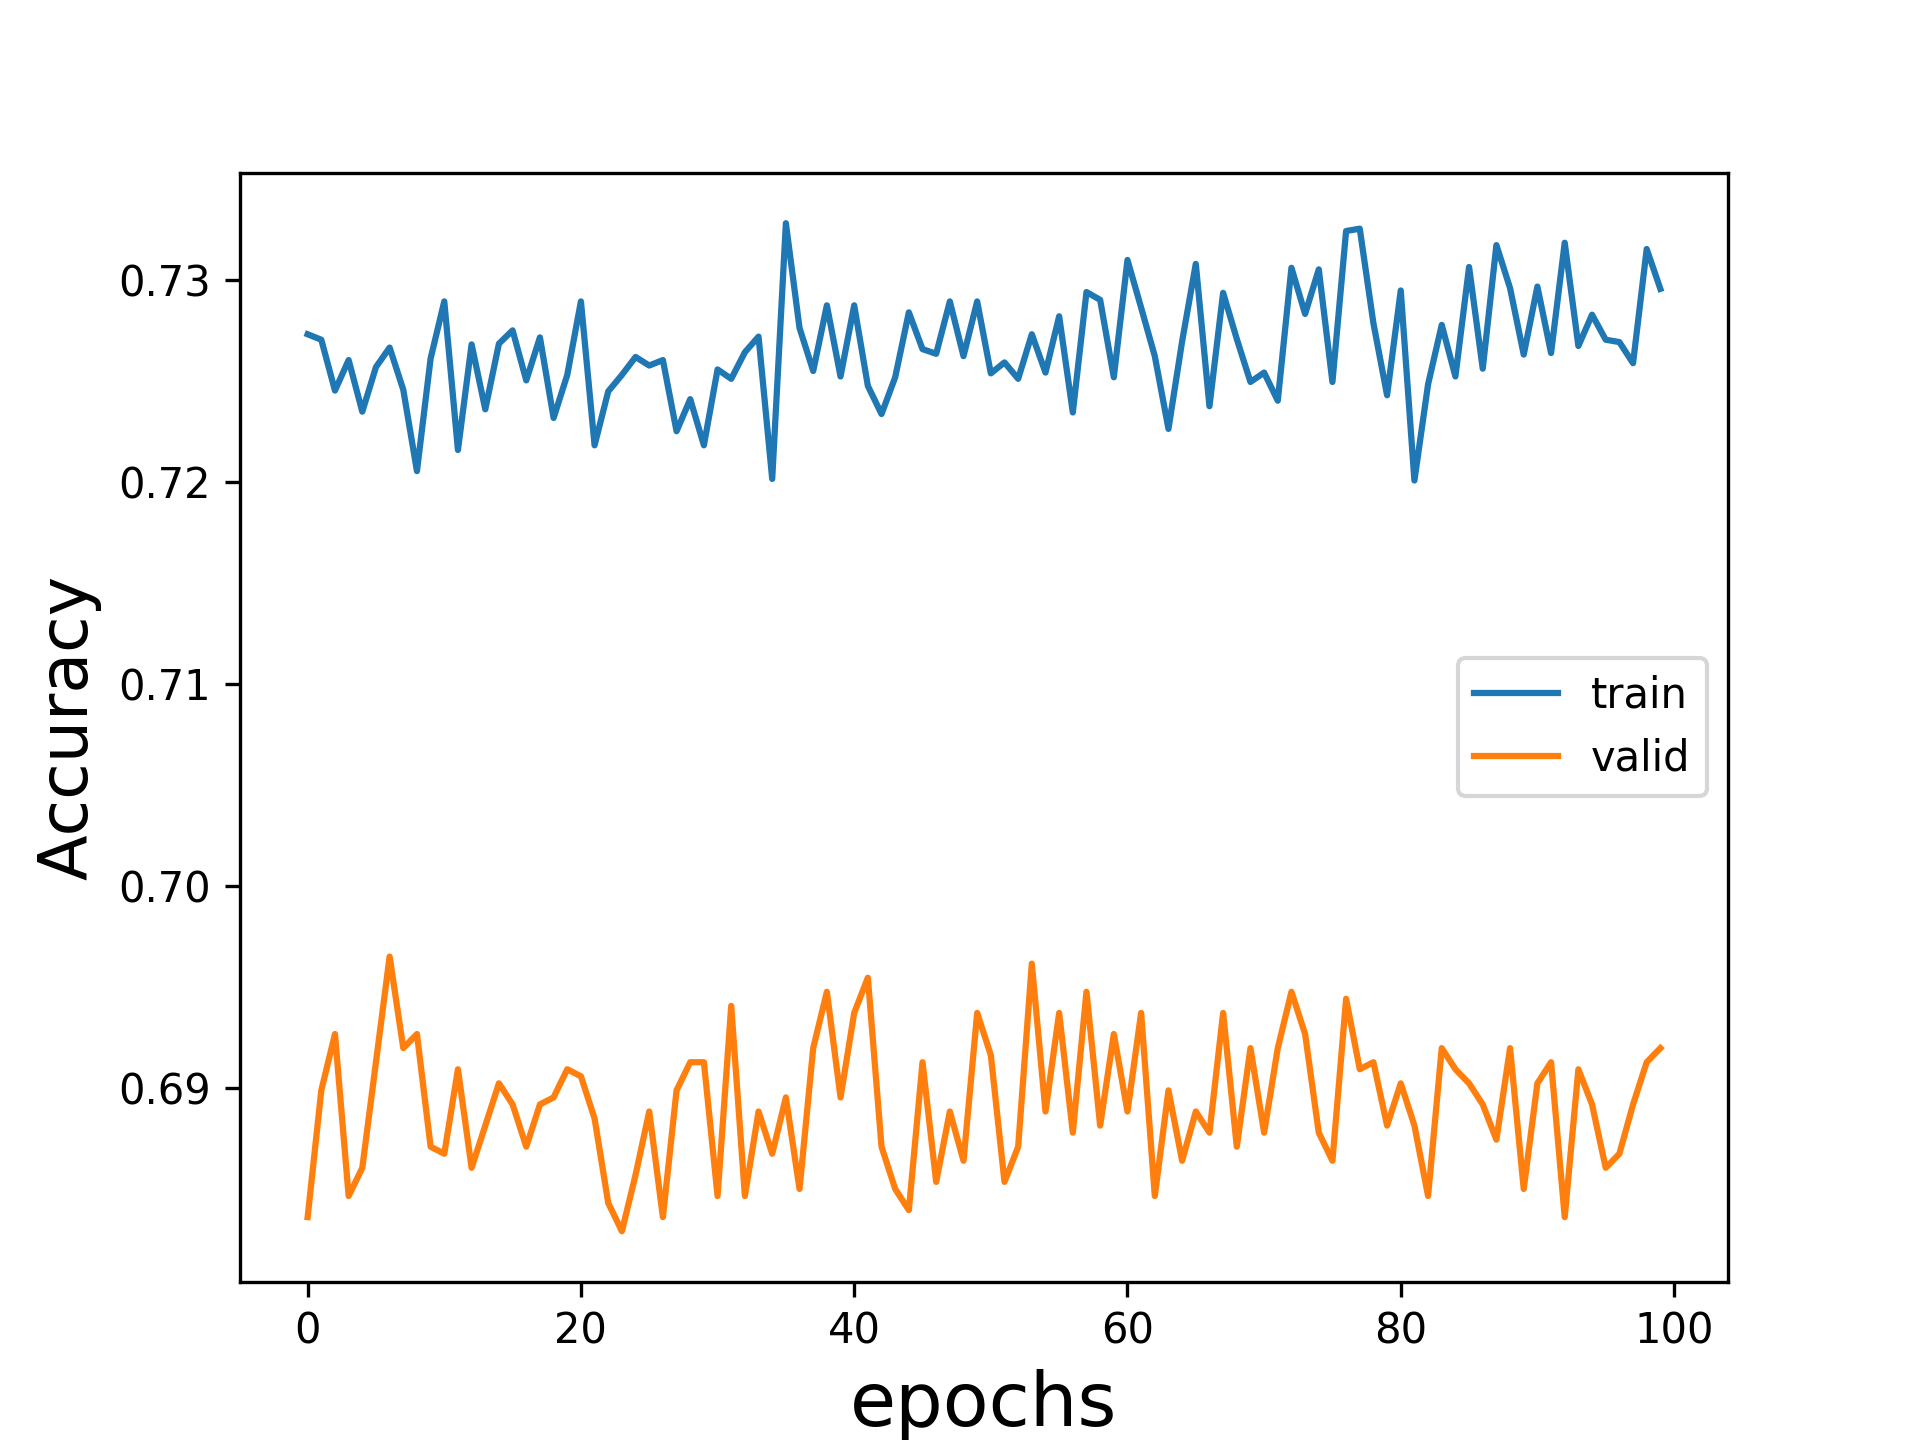
\includegraphics[width=\linewidth]{report-imgs/accuracy.png}
  \caption{Accuracy}
  \label{fig:sub1}
\end{subfigure}%
\begin{subfigure}{.5\textwidth}
  \centering
  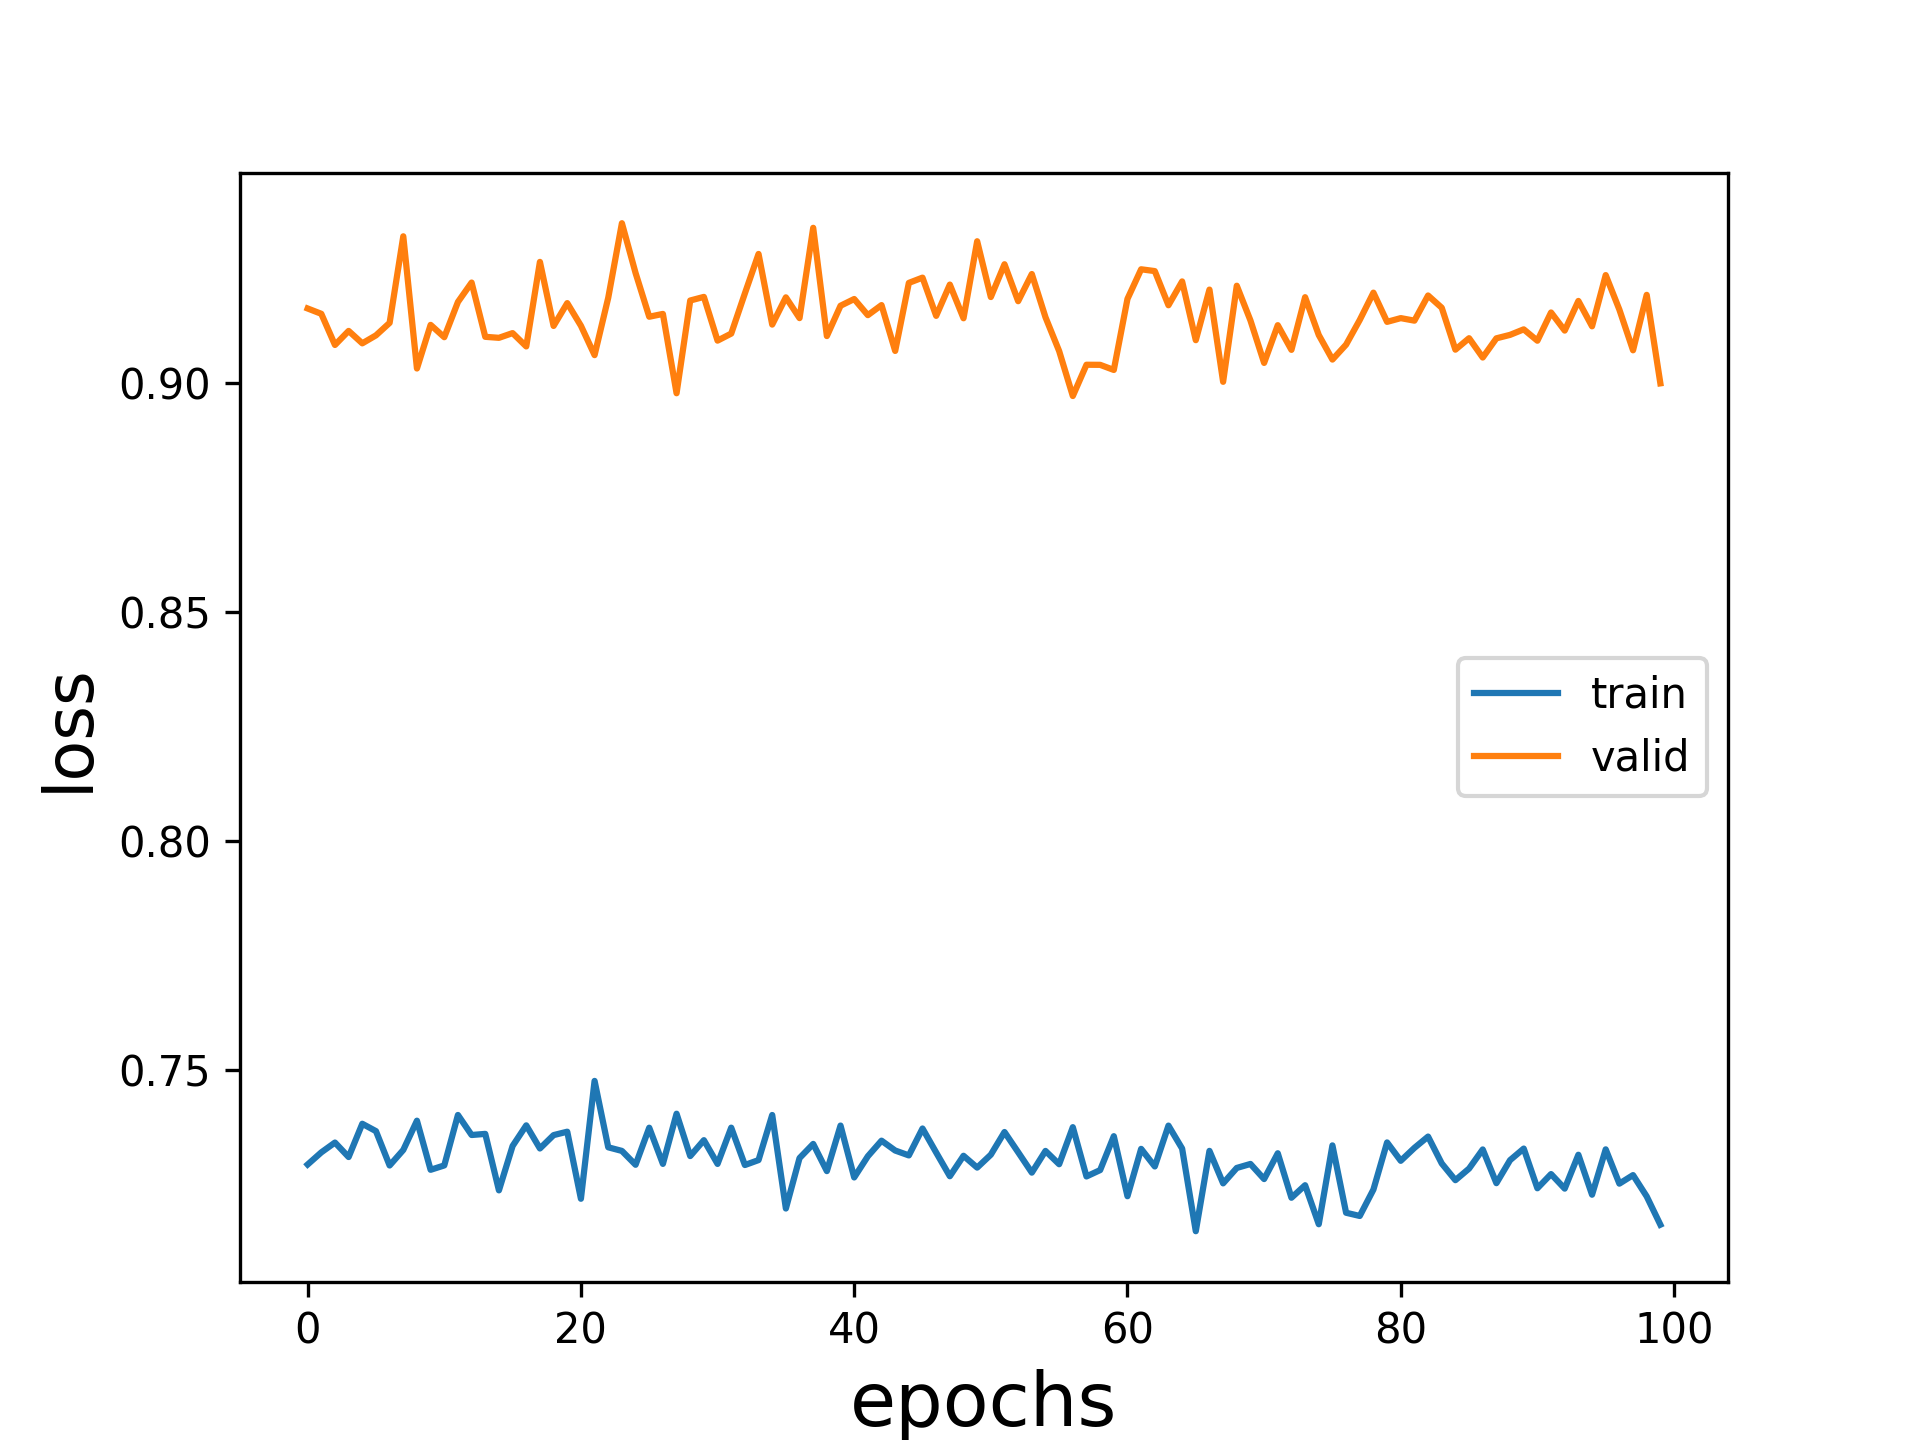
\includegraphics[width=\linewidth]{report-imgs/loss.png}
  \caption{Loss}
  \label{fig:sub2}
\end{subfigure}
\caption{Training Procedure}
\label{fig:test}
\end{figure}

\subsubsection*{Experiments}

The same structure without image augmentation is also tried. As shown below, it overfit severely start from about 10 epochs. Therefore, image augmentation is necessary to get higher accuracy.

\begin{figure}[H]
\centering
\begin{subfigure}{.5\textwidth}
  \centering
  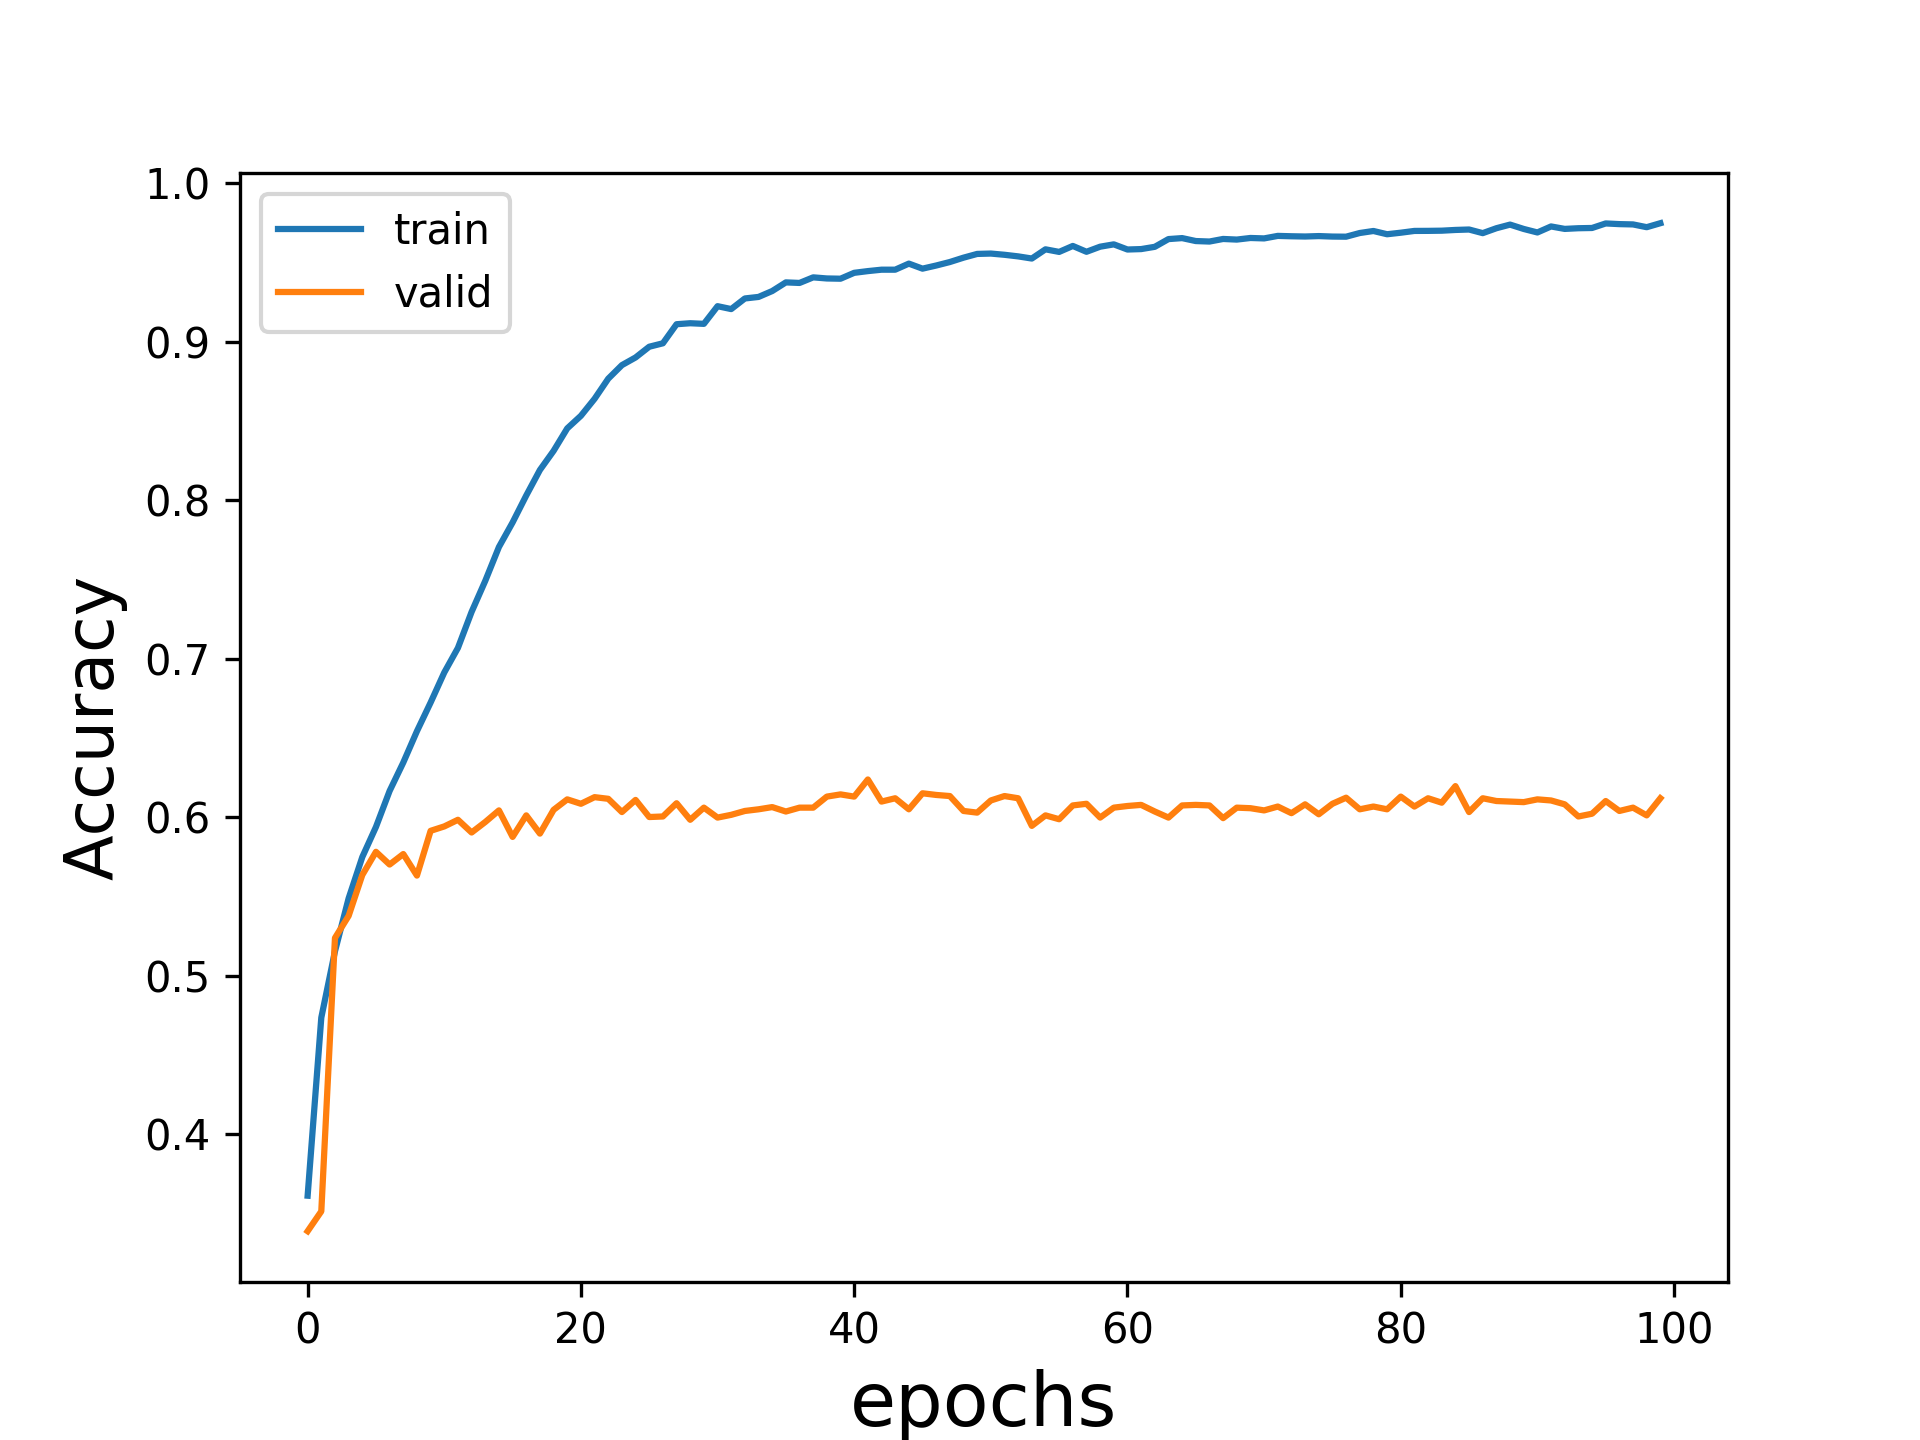
\includegraphics[width=\linewidth]{report-imgs/accuracy-without-aug.png}
  \caption{Accuracy}
  \label{fig:sub1}
\end{subfigure}%
\begin{subfigure}{.5\textwidth}
  \centering
  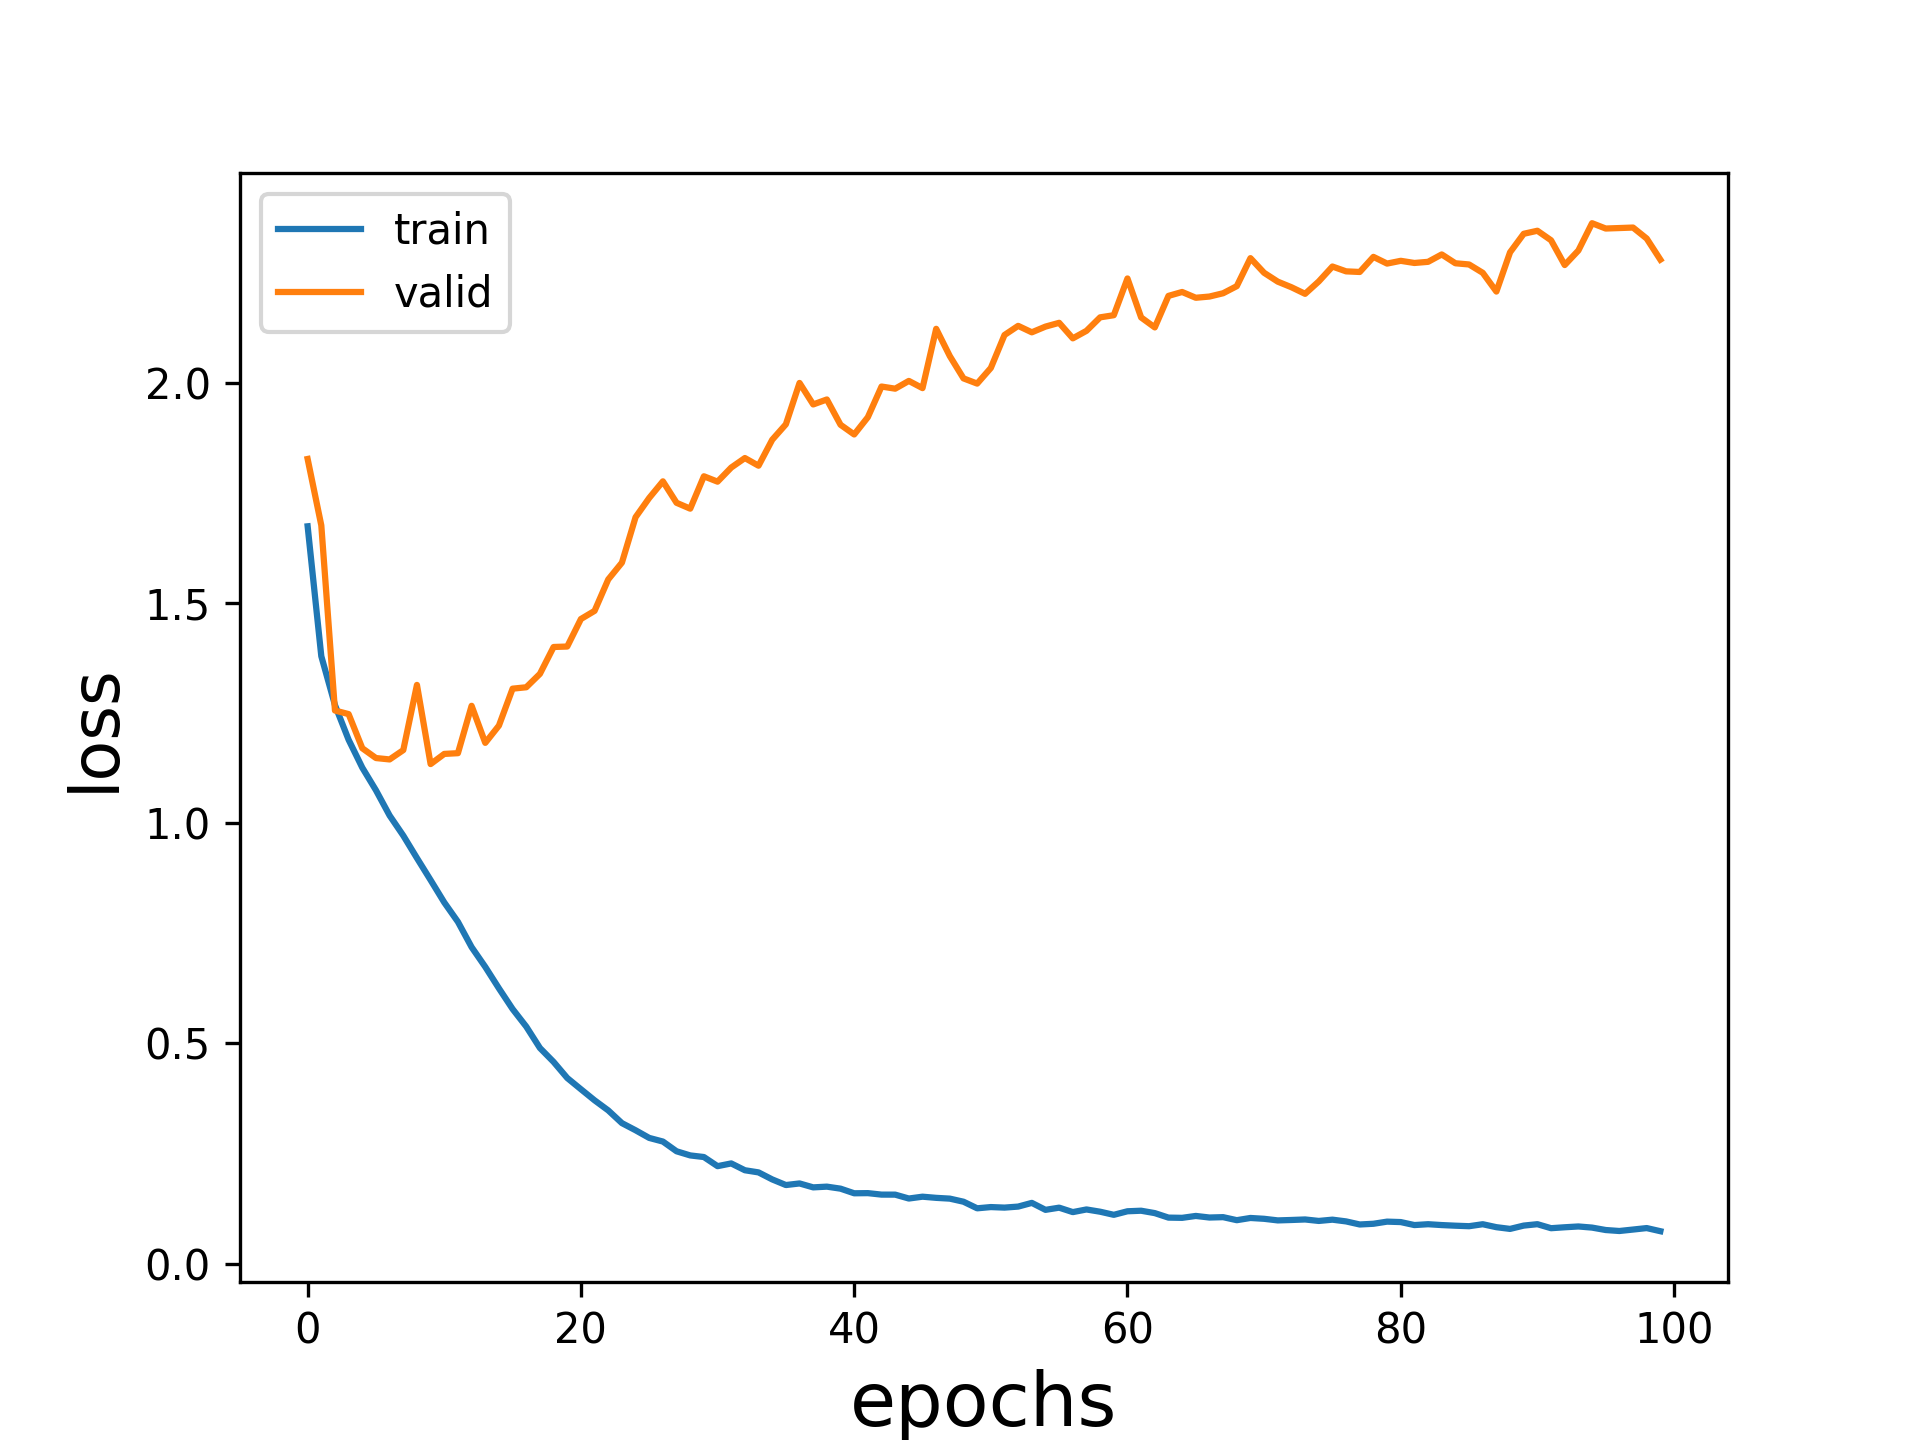
\includegraphics[width=\linewidth]{report-imgs/loss-without-aug.png}
  \caption{Loss}
  \label{fig:sub2}
\end{subfigure}
\caption{Training Procedure Without Image Augmentation}
\label{fig:test}
\end{figure}


\subsection*{P2: Build Deep Neural Network}

To compare with CNN model, I built a DNN model with same number of layers and approximately same number of parameters. The structure of DNN model is described bellow:

\begin{itemize}
\item Input (48, 48, 1)
\item Flatten (2304)
\item Dense (512), followed by batch normalization and leaky ReLU.
\item Dense (512), followed by batch normalization and leaky ReLU.
\item Dropout with drop rate 0.1.
\item Dense (512), followed by batch normalization and leaky ReLU.
\item Dropout with drop rate 0.1.
\item Dense (256), followed by batch normalization and leaky ReLU.
\item Dropout with drop rate 0.1.
\item Dense (256), followed by batch normalization and leaky ReLU.
\item Dropout with drop rate 0.1.
\item Dense (256), followed by batch normalization and leaky ReLU.
\item Dropout with drop rate 0.1.
\item Dense (7), followed by activation function softmax.
\end{itemize}

There are 1974791 trainable parameters, while for CNN model, there are 1703623 parameters.

As shown in figure 3, it is very hard for the DNN model to fit. Even after 1000 epochs, the training loss and accuracy still can hardly catch up with validation. In comparison, for the CNN model, the training loss gets lower than validation loss start from about 210 epochs. If the accuracy is compared, apparently CNN model is much more powerful. 

\begin{figure}[H]
\centering
\begin{subfigure}{.5\textwidth}
  \centering
  \includegraphics[width=\linewidth]{report-imgs/dnn-accuracy.png}
  \caption{Accuracy}
  \label{fig:sub1}
\end{subfigure}%
\begin{subfigure}{.5\textwidth}
  \centering
  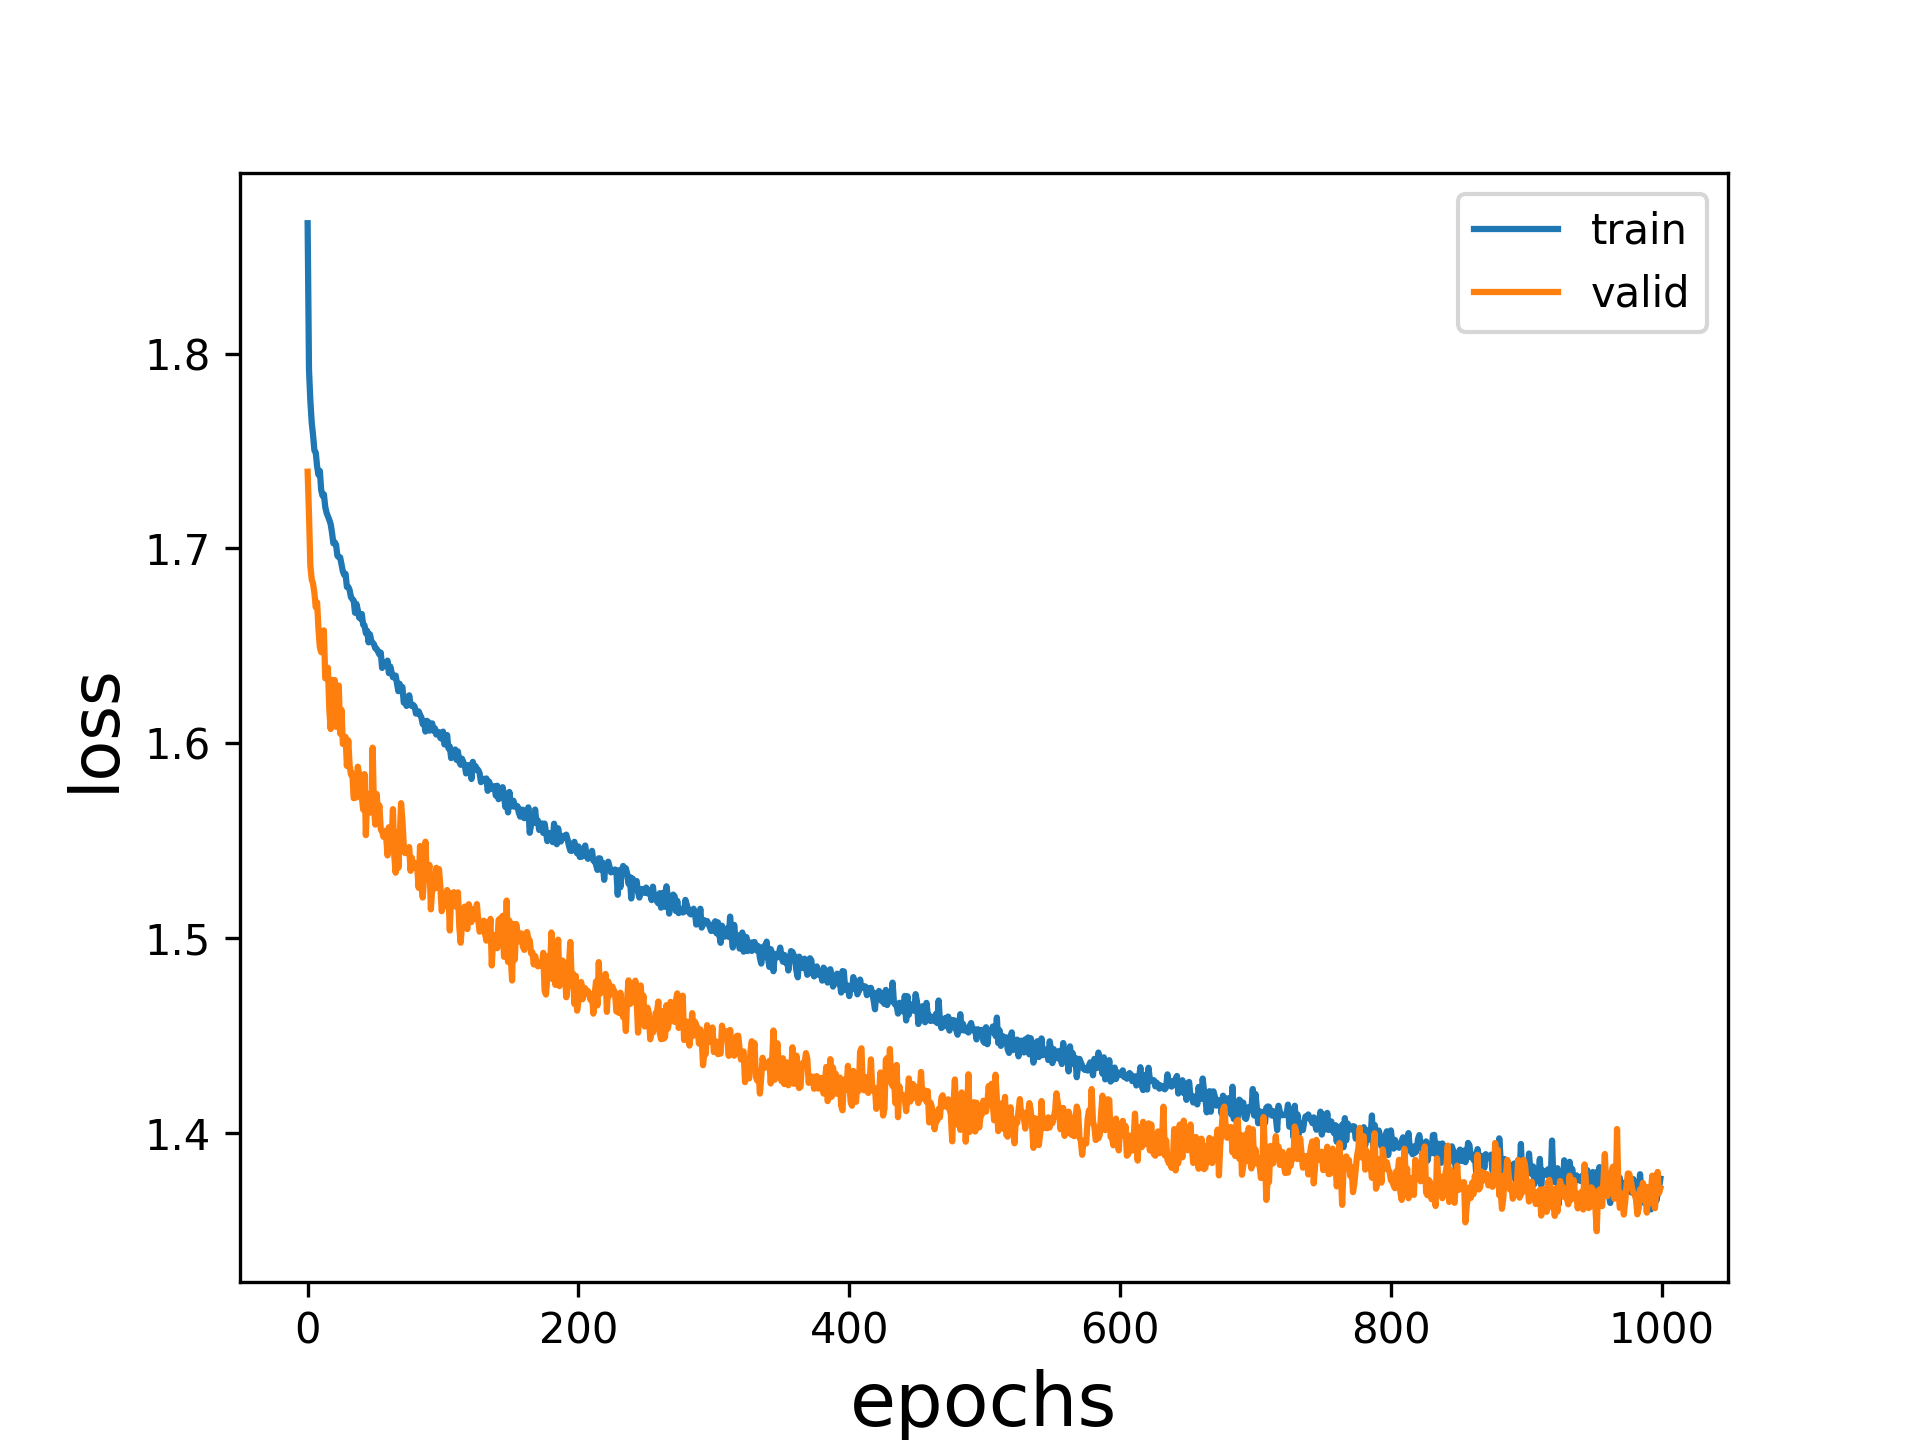
\includegraphics[width=\linewidth]{report-imgs/dnn-loss.png}
  \caption{Loss}
  \label{fig:sub2}
\end{subfigure}
\caption{Training Procedure of DNN}
\label{fig:test}
\end{figure}


\subsection*{P3: Analyze the Model by Confusion Matrix}

\begin{figure}[H]
\centering
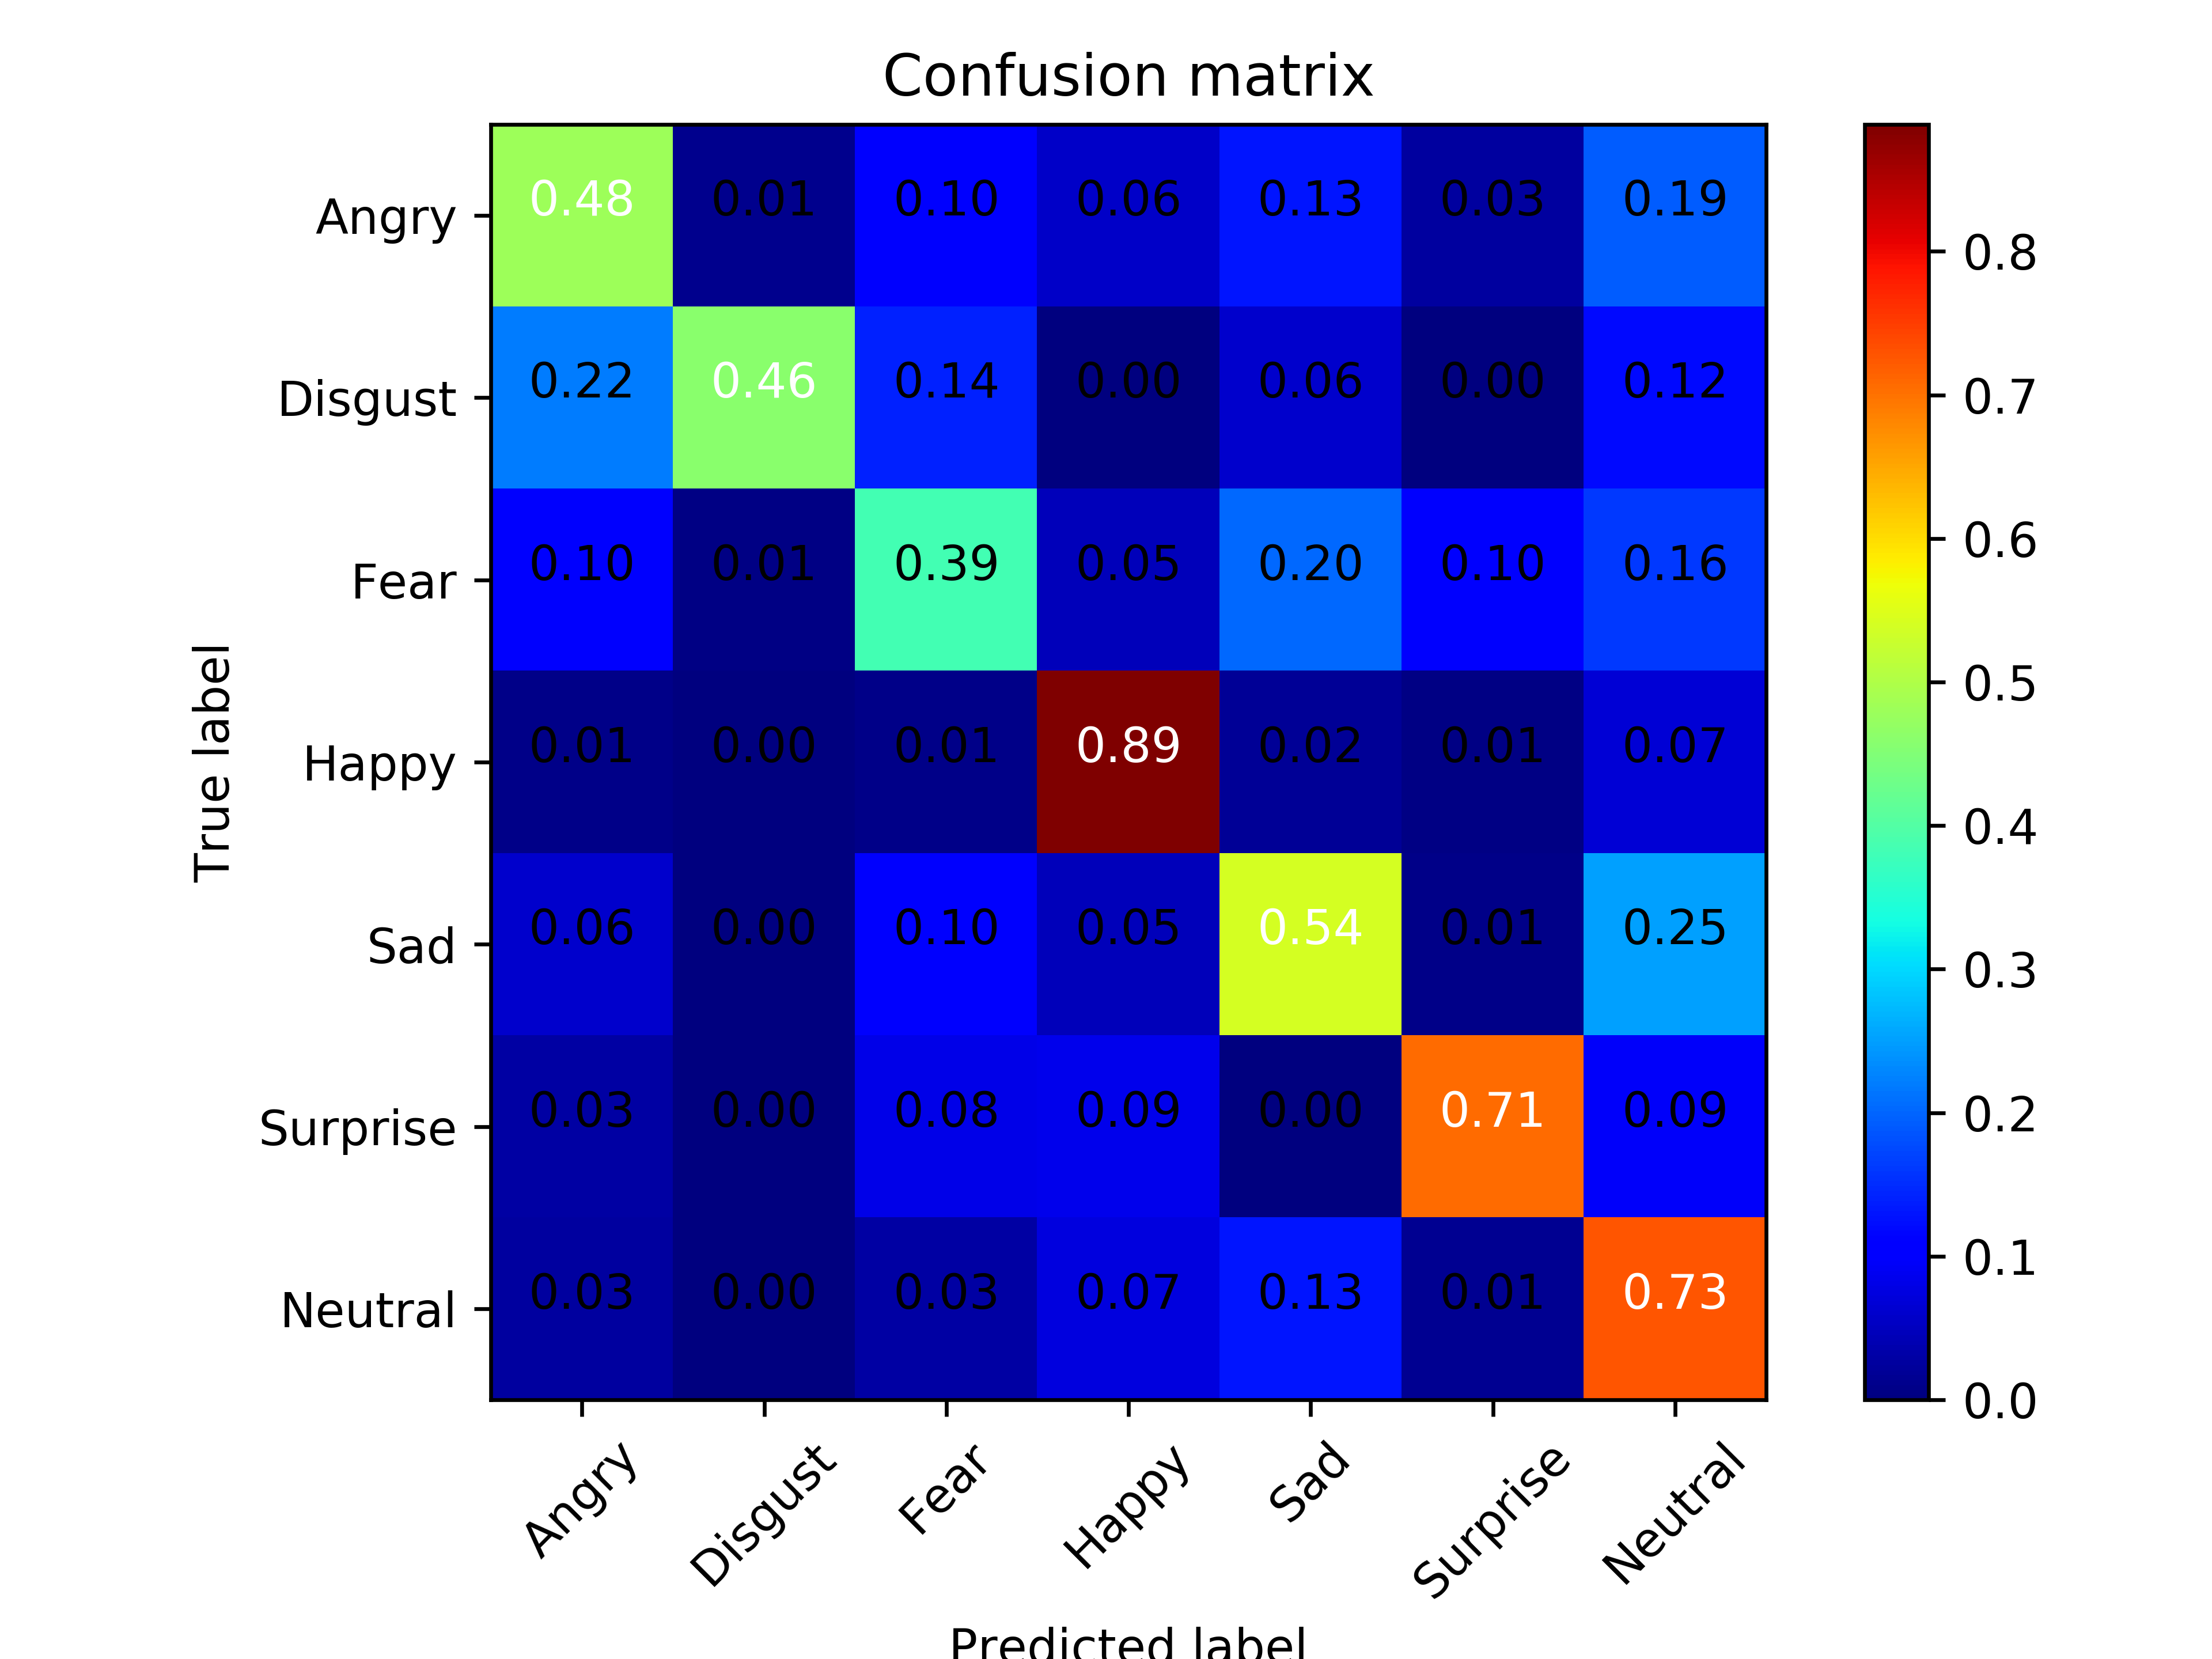
\includegraphics[width=\linewidth]{report-imgs/confusion.png}
\caption{Confusion Matrix}
\label{fig:confusion}
\end{figure}

As shown in Figure \ref{fig:confusion}, happy is the most easy facial expression to identify for the model, while fear is the most difficult. Also, 25\% of sad expressions is identify as neutral. That may implies that the facial expression of sad is not very apparent. 

\subsection*{P4: Analyze the Model by Plotting the Saliency Map}

The figures below are the saliency map of my CNN on figure 4 in the test data set. The heatmap is generate by calculating absolute value of gradient. From the image where low heat pixels are removed, we can identify the facial expression easily. Also, most part of the mouth is preserved. Therefore, the shape of mouth should be a important feature for the model to distinguish facial expression.

\begin{figure}[H]
\centering
\begin{subfigure}{.33\textwidth}
  \centering
  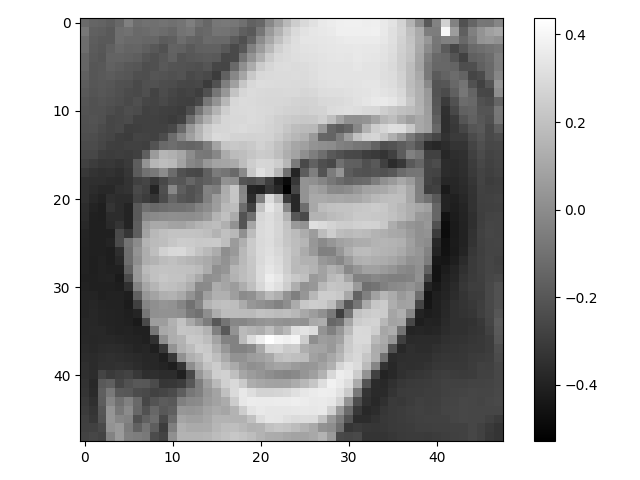
\includegraphics[width=\linewidth]{report-imgs/sa-orig.png}
  \caption{Original Image}
  \label{fig:sub1}
\end{subfigure}%
\begin{subfigure}{.33\textwidth}
  \centering
  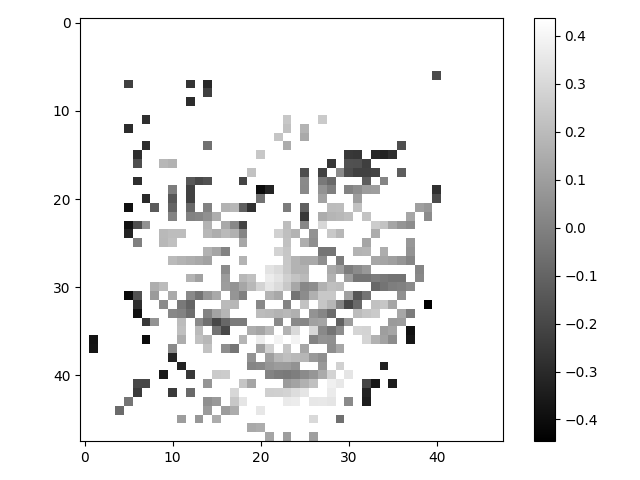
\includegraphics[width=\linewidth]{report-imgs/sa-rm-low-heat.png}
  \caption{Remove low heat}
  \label{fig:sub2}
\end{subfigure}
\begin{subfigure}{.33\textwidth}
  \centering  
  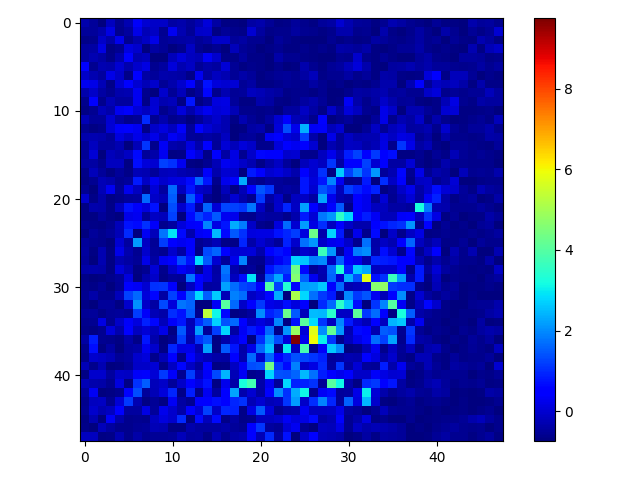
\includegraphics[width=\linewidth]{report-imgs/sa.png}
  \caption{Saliency Map}
  \label{fig:sub1}
\end{subfigure}%
\caption{Training Procedure}
\label{fig:test}
\end{figure}


\subsection*{P5: Analyze the Model by Visualizing Filters}

Following images are the output of filters in layer 2 and images that activate those filters most. From the output of those filters, we can identify organs such as eye, eyebrow, mouth. Thus those filters seem to try to mark those facial organs in different ways. Also, some filters seem to be complementary, such as filter 25 and 26, while some of them are very similar. The similarity between filters may imply that number of filters is more than necessary. However, those redundant filters may provides better ability to resist noise.

From the images that activate the filters most, we can barely find any information. The reason may be that, those filters are to find more subtle features of part of organs, while they are too obscure to our human beings.

The second layer of another model, referred as dlsvm, proposed by the winner of FER 2013 \cite{dlsvm}, can be compared here. For this model I can only tune to about 65\% accuracy. As shown in figure, some filters, such as filter 26, are also trying to mark those organs. However, apparently its filters preserve less features and less delicate. That may be reasonable since it has less number of layers.


\begin{figure}[H]
  \centering
  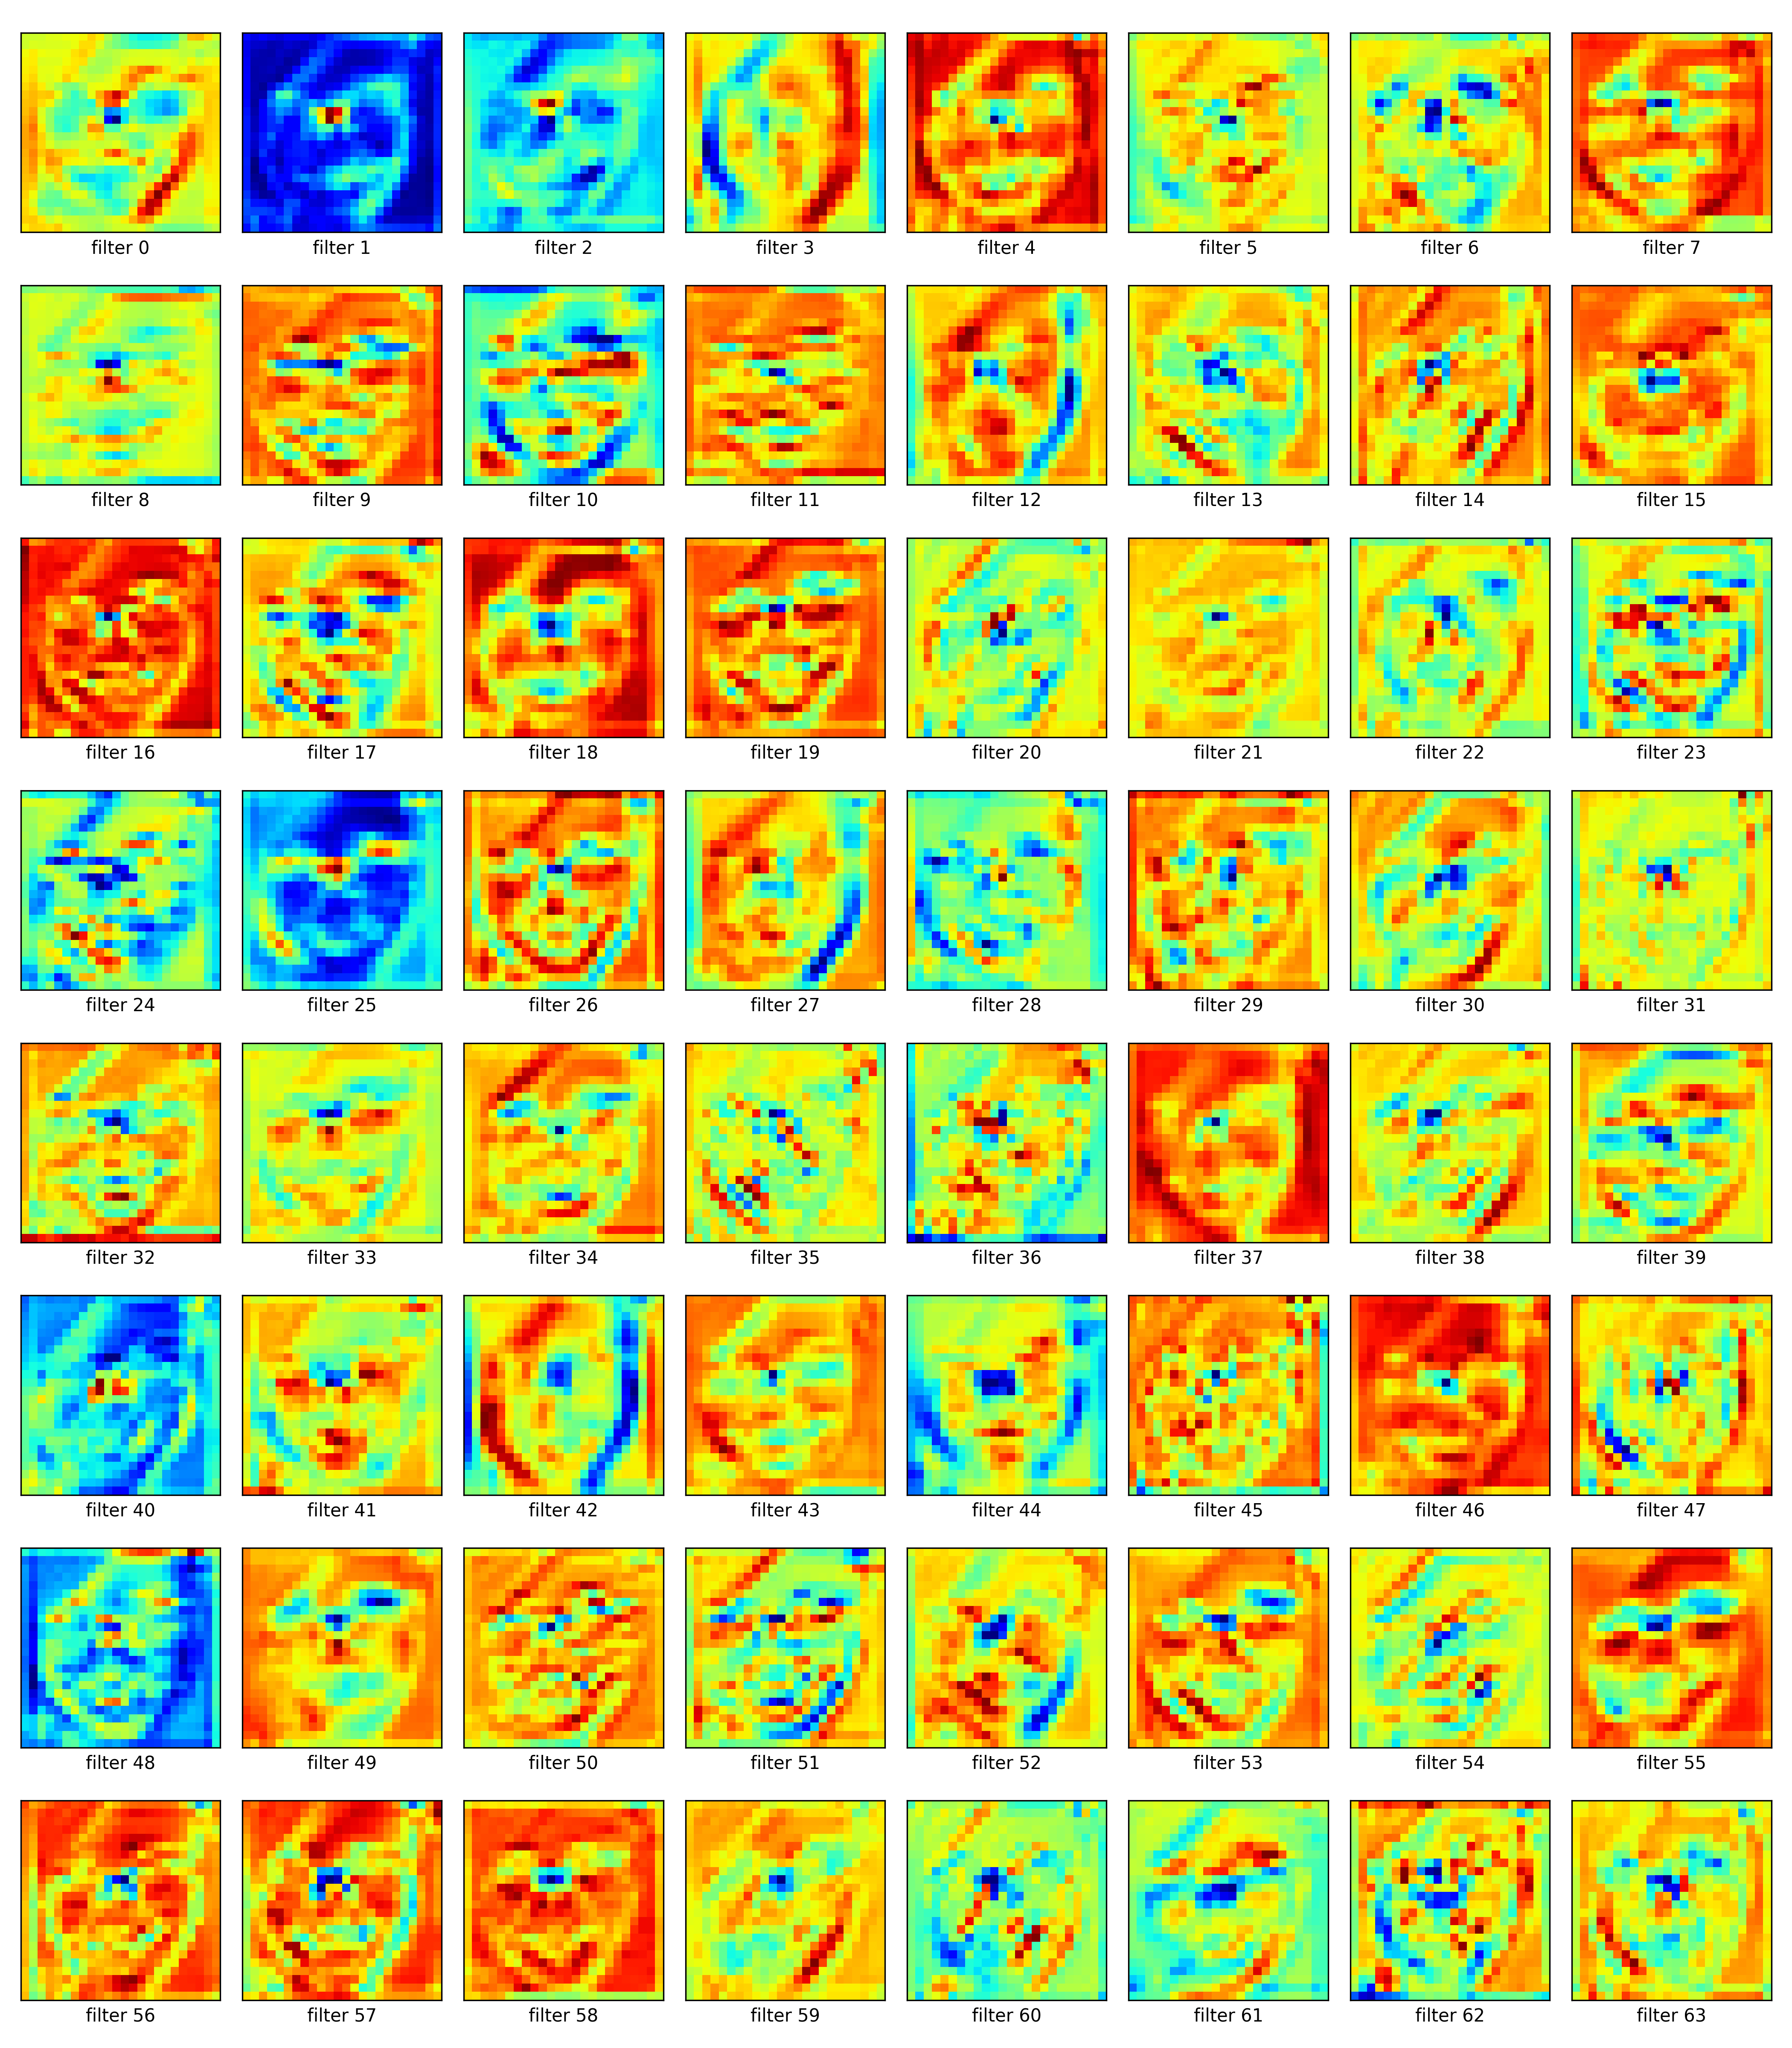
\includegraphics[width=\linewidth]{report-imgs/filter-output.png}
  \caption{Output of filters in layer 2}
  \label{fig:Output of filters in layer 2}
\end{figure}

\begin{figure}[H]
  \centering
  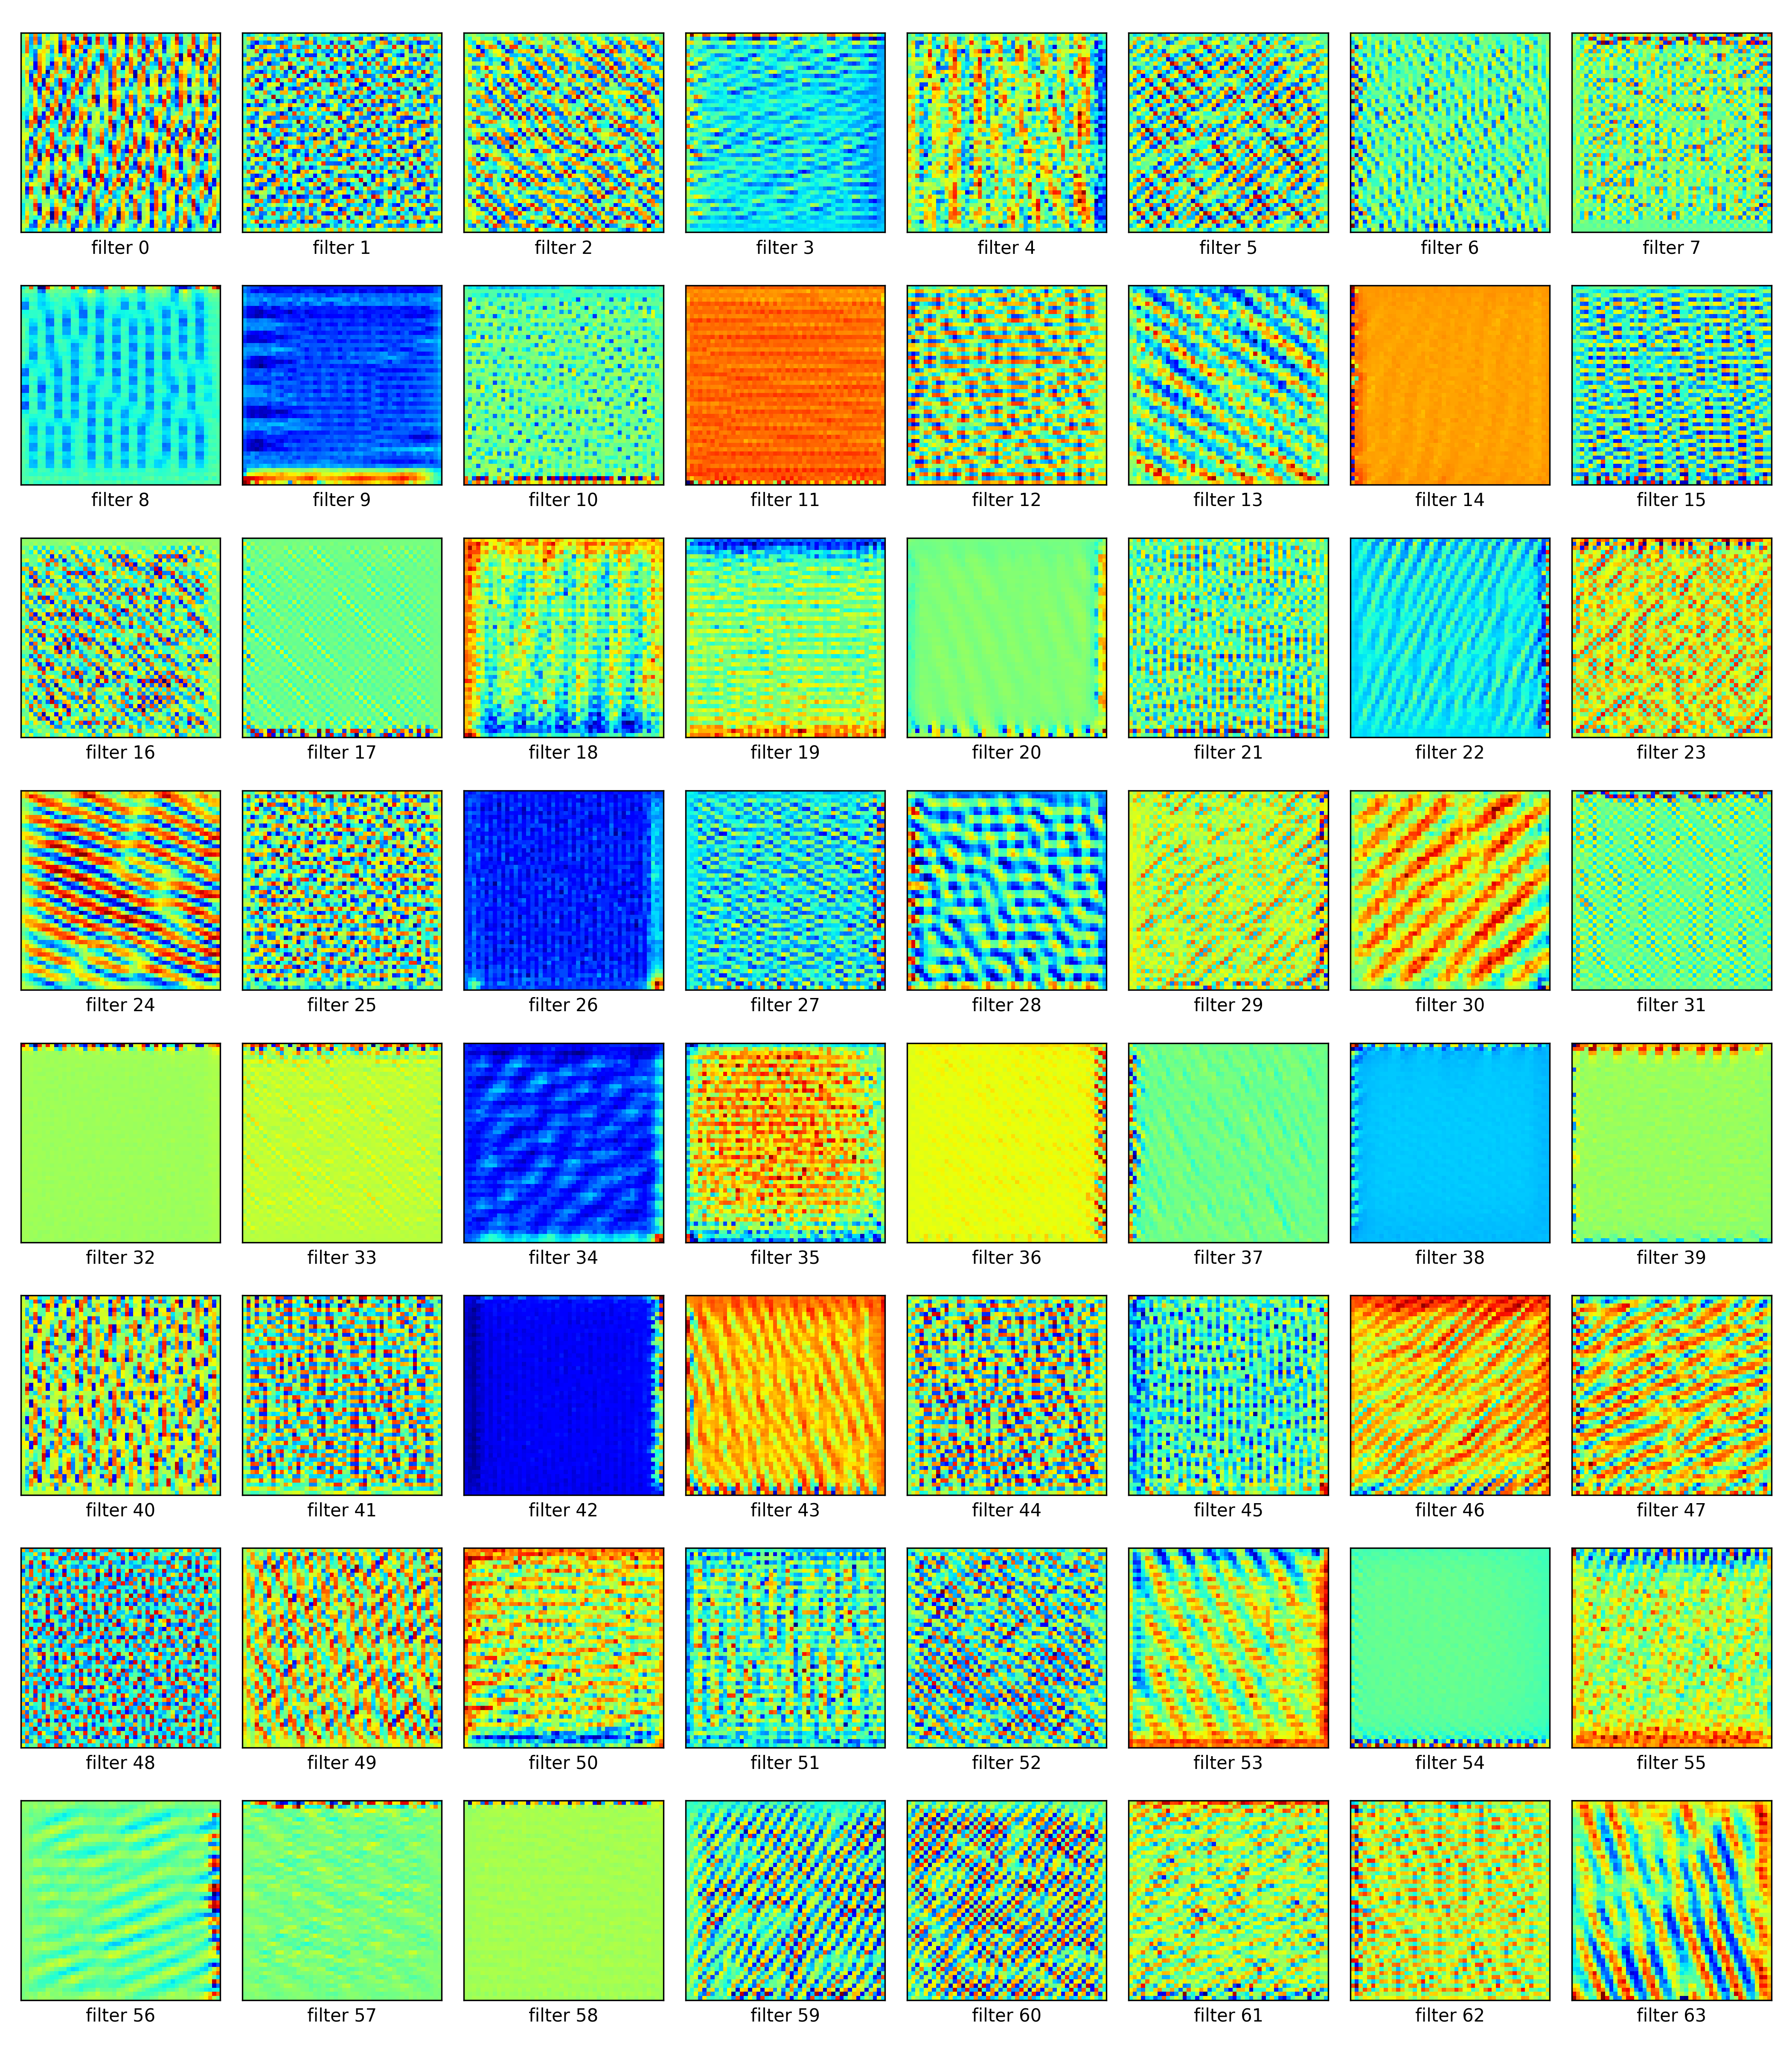
\includegraphics[width=\linewidth]{report-imgs/filter-visualize.png}
  \caption{Visualization of filters in layer 2}
  \label{fig:Visualization of filters in layer 2}
\end{figure}


\begin{figure}[H]
  \centering
  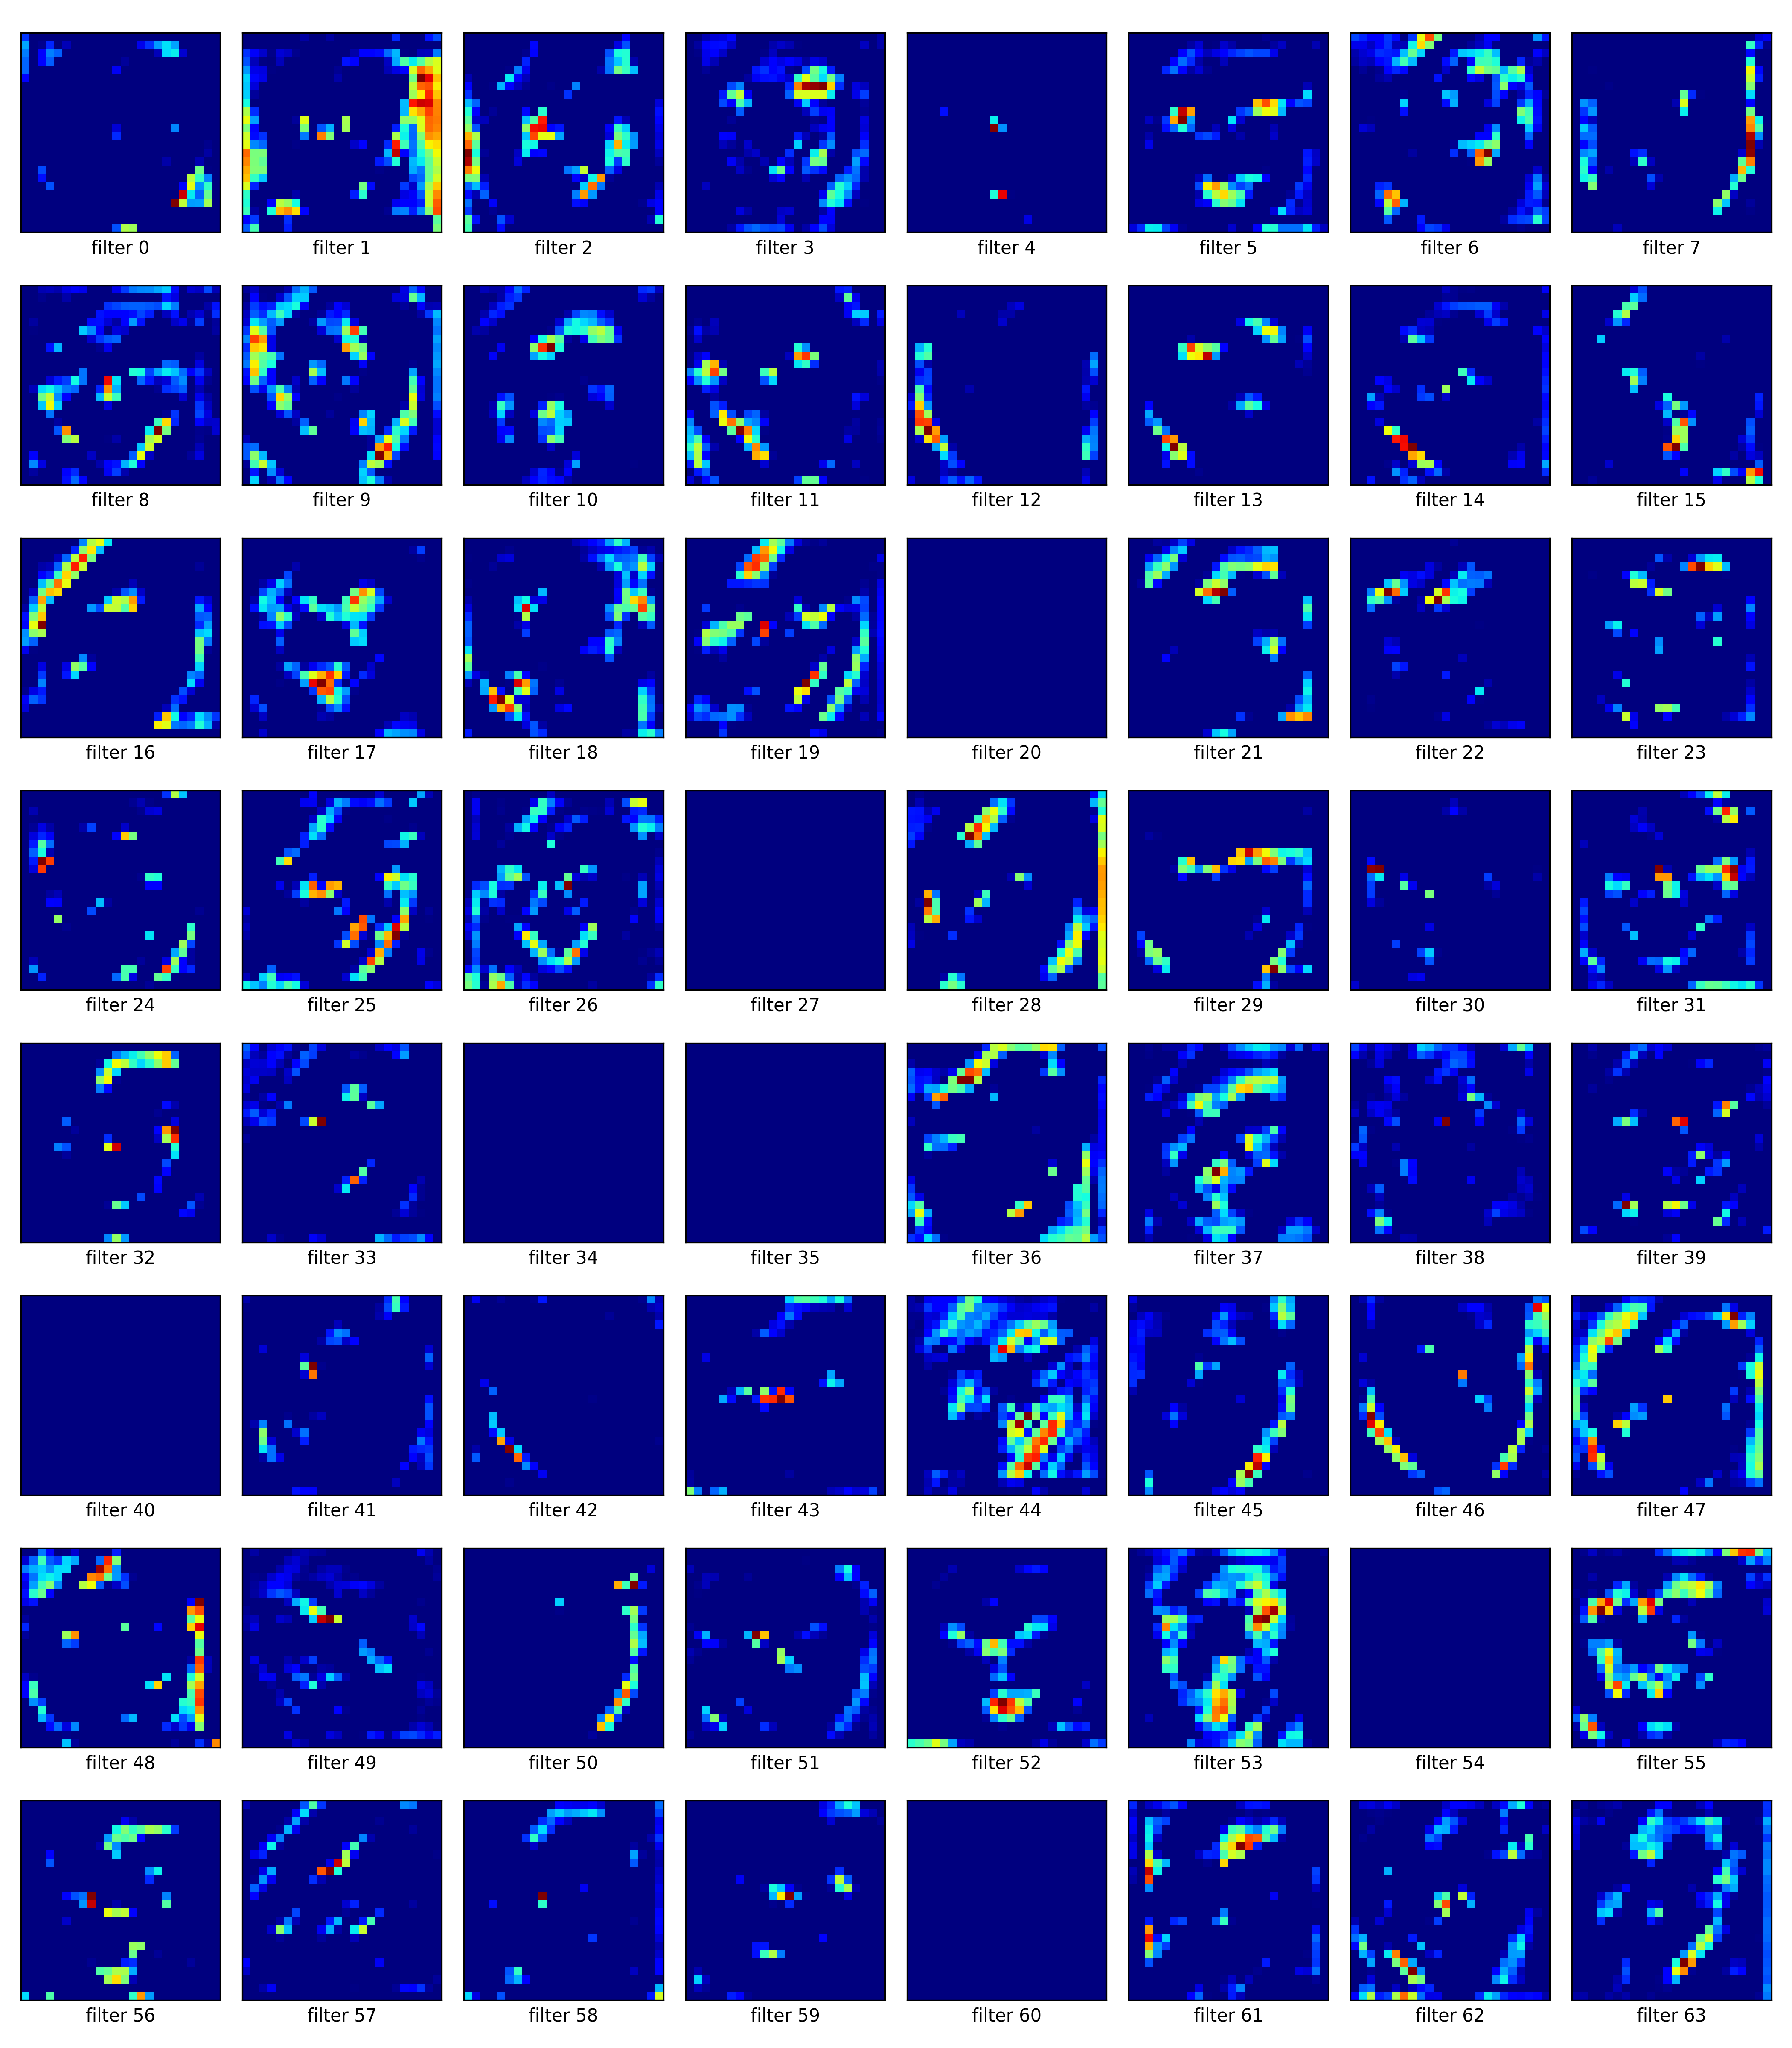
\includegraphics[width=\linewidth]{report-imgs/dlsvm-filter-output.png}
  \caption{DLSVM: Output of filters in layer 2}
  \label{fig:Output of filters in layer 2}
\end{figure}


\subsection*{Bonus: Semi-supervied Learning}

Semi-supervised learning was also tried. The training procedure is bellow.

\begin{itemize}
\item Split 10\% validation data from training data.
\item Train the model with the 90\% data remained for 600 epochs.
\item Predict on test data. Pick top 10\% most confident prediction from test data and merge them into training data. Fit for 50 epochs.
\item Repeat the step above for 10 times.
\end{itemize}

As shown in figure \ref{fig:semi}, as test data is added, training accuracy increases faster and training loss drop faster too. Also, valid accuracy drops a little bit, while valid loss oscillates severely. Overall, the performance did not differ much compared with the original one.

\begin{figure}[H]
\centering
\begin{subfigure}{.5\textwidth}
  \centering
  \includegraphics[width=\linewidth]{report-imgs/semi-accuracy.png}
  \caption{Accuracy}
  \label{fig:sub1}
\end{subfigure}%
\begin{subfigure}{.5\textwidth}
  \centering
  \includegraphics[width=\linewidth]{report-imgs/semi-loss.png}
  \caption{Loss}
  \label{fig:sub2}
\end{subfigure}
\caption{Training Procedure}
\label{fig:semi}
\end{figure}


\clearpage

\begin{thebibliography}{99}
\bibitem{cs221_project} 
Mo, Kaichun, Yang, Yuxin, Zhang, Yun. CS  221  Project  Final  Report:  Facial  Expression  Automatic  Recognition. http://www.cs.stanford.edu/~kaichun/resume/cs221\_project\_report.pdf
\bibitem{dlsvm} 
Yichuan Tang. Deep Learning using Linear Support Vector Machines.  
\end{thebibliography}

\end{document}
